\subsection{Imagination, Searching, Criticizing and Learning Loop}
% ALGORITHM STYLE -- Released 8 April 1996
%    for LaTeX-2e
% Copyright -- 1994 Peter Williams
% E-mail Peter.Williams@dsto.defence.gov.au
\NeedsTeXFormat{LaTeX2e}
\ProvidesPackage{algorithm}
\typeout{Document Style `algorithm' - floating environment}

\RequirePackage{float}
\RequirePackage{ifthen}
\newcommand{\ALG@within}{nothing}
\newboolean{ALG@within}
\setboolean{ALG@within}{false}
\newcommand{\ALG@floatstyle}{ruled}
\newcommand{\ALG@name}{Algorithm}
\newcommand{\listalgorithmname}{List of \ALG@name s}

% Declare Options
% first appearance
\DeclareOption{plain}{
  \renewcommand{\ALG@floatstyle}{plain}
}
\DeclareOption{ruled}{
  \renewcommand{\ALG@floatstyle}{ruled}
}
\DeclareOption{boxed}{
  \renewcommand{\ALG@floatstyle}{boxed}
}
% then numbering convention
\DeclareOption{part}{
  \renewcommand{\ALG@within}{part}
  \setboolean{ALG@within}{true}
}
\DeclareOption{chapter}{
  \renewcommand{\ALG@within}{chapter}
  \setboolean{ALG@within}{true}
}
\DeclareOption{section}{
  \renewcommand{\ALG@within}{section}
  \setboolean{ALG@within}{true}
}
\DeclareOption{subsection}{
  \renewcommand{\ALG@within}{subsection}
  \setboolean{ALG@within}{true}
}
\DeclareOption{subsubsection}{
  \renewcommand{\ALG@within}{subsubsection}
  \setboolean{ALG@within}{true}
}
\DeclareOption{nothing}{
  \renewcommand{\ALG@within}{nothing}
  \setboolean{ALG@within}{true}
}
\DeclareOption*{\edef\ALG@name{\CurrentOption}}

% ALGORITHM
%
\ProcessOptions
\floatstyle{\ALG@floatstyle}
\ifthenelse{\boolean{ALG@within}}{
  \ifthenelse{\equal{\ALG@within}{part}}
     {\newfloat{algorithm}{htbp}{loa}[part]}{}
  \ifthenelse{\equal{\ALG@within}{chapter}}
     {\newfloat{algorithm}{htbp}{loa}[chapter]}{}
  \ifthenelse{\equal{\ALG@within}{section}}
     {\newfloat{algorithm}{htbp}{loa}[section]}{}
  \ifthenelse{\equal{\ALG@within}{subsection}}
     {\newfloat{algorithm}{htbp}{loa}[subsection]}{}
  \ifthenelse{\equal{\ALG@within}{subsubsection}}
     {\newfloat{algorithm}{htbp}{loa}[subsubsection]}{}
  \ifthenelse{\equal{\ALG@within}{nothing}}
     {\newfloat{algorithm}{htbp}{loa}}{}
}{
  \newfloat{algorithm}{htbp}{loa}
}
\floatname{algorithm}{\ALG@name}

\newcommand{\listofalgorithms}{\listof{algorithm}{\listalgorithmname}}


The algorithm is shown in Algorithm~\ref{algo:self_improving}.

\subsection{Option-level MCTS}
\label{app:option_level_mcts}
\begin{figure}[!t]
    \centering
    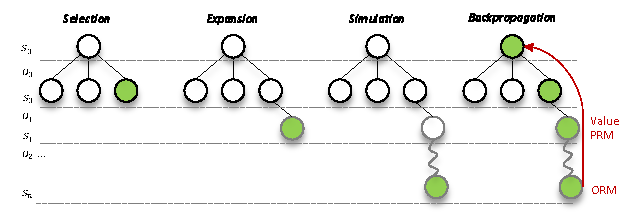
\includegraphics[width=\textwidth]{figures/emcts.pdf}
    \caption{An overview of the four operations of \emcts{}. A node is selected, expanded, simulated with fast rollout policy until a terminal node is reached, then the signals from value function, \prm{} and \orm{} are backpropagated.}
    \label{fig:emcts}
\end{figure}
As illustrated in Figure~\ref{fig:emcts}, option-level MCTS consists of the following operations:
\begin{itemize}[noitemsep,topsep=0pt,parsep=2pt,partopsep=0pt,leftmargin=*]
\item \textbf{Selection} Starting from the root node, we iteratively select the child node based on Equation \ref{eqs:ucb}.
\item \textbf{Expansion} Once an expandable leaf node is selected, a new node is generated by starting with the previous state of the parent node as the initial option state. The option is then sampled using the policy $\pi$, and its completion is determined by the termination function $\beta$. 
\item \textbf{Simulation} The scaled reward of the newly expanded node, as well as some simulated future trajectories are evaluated using the feedback functions, which is discussed in \S \ref{sec:critic}.
\item \textbf{Backpropagation} The average value of the newly generated node and all its ancestors is updated using the scaled reward from the evaluation step. Meanwhile, the visit counts for these nodes are also increased by one.
\end{itemize}


\subsection{Importance-Based Adaptive Branching Under Uniform Distribution}
\label{app:node_importance_uniform} 
\renewcommand{\thetheorem}{\ref{thm:optimal_branching_factor}}

Let $V = \{v_\phi^\pi(\vs_t, \vo_t^1), v_\phi^\pi(\vs_t, \vo_t^2), ..., v_\phi^\pi(\vs_t, \vo_t^{m_t})\}$ be a set of $m_t$ values that are uniformly distributed. If the maximum and minimum values from $V$ are $v_{\max}$ and $v_{\min}$, the average gap between two consecutive values is given by $\frac{v_{\max} - v_{\min}}{m_t - 1}$. The upper bound of expected minimum distances from a new value $v_{\text{new}}$ to any value from $V$ is achieved when $v_{\text{new}}$ is consistently positioned at the midpoint between two consecutive values, and it is given by $\frac{v_{\max} - v_{\min}}{2(m_t - 1)}$.

Since $v_{\max} - v_{\min}=2I(\vs_t)$ for a uniform distribution, we can conclude that $E_\phi(t) \le \frac{I(\vs_t)}{m_t - 1}$.

\begin{theorem}
The optimal branching factor $m_t$ in a tree search is set such that $m_t - 1$ is proportional to the node importance $I(\vs_t)$, under the condition $\frac{I(\vs_t)}{m_t-1} \le \epsilon$.
\end{theorem}

\begin{proof}
We can have the optimization problem as:
\begin{align*}
\text{minimize:} & \sum m_t \\
\text{subject to:} & \frac{I(\vs_t)}{m_t-1} \le \epsilon
\end{align*}

Introduce the Lagrange multiplier $\lambda_t$ for each constraint:

$$
L(m_t, \lambda_t) = \sum m_t + \sum \lambda_t \left (\epsilon (m_t-1) - I(\vs_t)\right)
$$

Now, let's find the gradient of the Lagrangian with respect to $m_t$ and $\lambda_t$ and set them to zero:

\begin{align*}
\nabla_{m_t} L &= 1 + \epsilon \lambda_t = 0 \\
\nabla_{\lambda_t} L &= \epsilon (m_t-1) - I(\vs_t) = 0
\end{align*}

From the first equation, we get:

$$
\lambda_t = -\frac{1}{\epsilon}
$$

Substitute this value of $\lambda_t$ into the second equation:

$$
\epsilon (m_t-1) - I(\vs_t) = 0
$$

Solving for $m_t$, we get:

$$
m_t = \frac{I(\vs_t)}{\epsilon} + 1
$$

Thus, $m_t - 1$ is proportional to the node importance $I(\vs_t)$.
\end{proof}

\subsection{Importance-Based Adaptive Branching Under Gaussian Distribution}
\label{app:node_importance_gaussian} 

If we assume that \(v_{\phi}^{\pi}([\vs_t, \vo_t^{j}])\) and \(v_{\phi}^{\pi}([\vs_t, \vo_t^{i}])\) are independent and identically distributed Gaussian random variables:
\[
v_{\phi}^{\pi}([\vs_t, \vo_t^{j}]), v_{\phi}^{\pi}([\vs_t, \vo_t^{i}]) \sim \mathcal{N}(\mu, \sigma^2)
\]
The difference \(D_{ij} = v_{\phi}^{\pi}([\vs_t, \vo_t^{j}]) - v_{\phi}^{\pi}([\vs_t, \vo_t^{i}])\) will follow a normal distribution with:
\[
D_{ij} \sim \mathcal{N}(0, 2\sigma^2)
\]
To find the expected minimum absolute difference between \(v_{\phi}^{\pi}([\vs_t, \vo_t^{j}])\) and the closest \(v_{\phi}^{\pi}([\vs_t, \vo_t^{i}])\), we need to consider the distribution of the minimum of \(m_t\) Gaussian differences.

The expected minimum value of \(m_t\) absolute differences can be approximated using properties of order statistics for Gaussian distributions.

For a set of \(m_t\) independent normal random variables with variance \(2\sigma^2\), the expected minimum absolute difference, \(\mathbb{E}[\min_{i} |D_{ij}|]\), can be approximated by:
\[
E_{\phi}(t) \approx \frac{\sigma \sqrt{2}}{\sqrt{m_t}}
\]
This approximation arises from the fact that the expected minimum value of the absolute deviations of normally distributed random variables scales with the inverse of the square root of the number of samples.

Then, assume the range of the $m_t$ samples are $R_m=max(v_{\phi}^{\pi}([\vs_t, \vo_t^{i}])-min(v_{\phi}^{\pi}([\vs_t, \vo_t^{i}])$, the the expected range \( \mathbb{E}[R_m] \) of \( m_t \) samples from a normal distribution can be approximated using properties of extreme values of Gaussian distributions.
The range \( R_m \) can be approximated as:
\[
R_m \approx \sigma (z_{0.9995} - z_{0.0005})
\]
where \( z_{p} \) is the p-th percentile of the standard normal distribution. It can converge to 
\[
R_m \approx \sigma \sqrt{2 \ln(m_t)} \left( 2 - \frac{\ln(\ln(m_t))}{4 \ln(m_t)} \right)
\]
For simplicity, we can approximate the range using the primary term, which captures the dominant behavior:
\[
R_m \approx \sigma \sqrt{2 \ln(m_t)}
\]
Then we have 
\[
E_{\phi}(t) \approx \frac{\sqrt{2}}{{\sqrt{m_t}}}\frac{R_m}{\sqrt{2 \ln(m_t)}}
\]
Knowing that for all distributions, 
\[
I(\vs_t) \ge \frac{R_m}{2}
\]
We have 
\[
E_{\phi}(t) \le \frac{I(s_t)}{\sqrt{m_t\ln(m_t)}}
\]
Then to find the optimal $m_t$, the optimization problem is
\begin{align*}
\text{minimize:} & \sum m_t \\
\text{subject to:} & \frac{I(s_t)}{\sqrt{m_t\ln(m_t)}} \leq \epsilon
\end{align*}

To solve this optimization problem, we can first rewrite the constraint in terms of $m_t$.
\[
m_t\ln(m_t) \geq \frac{I^2(s_t)}{\epsilon^2}
\]

Now, let's define a new function $g(m_t) = m_t\ln(m_t)$. We want to find the minimum $m_t$ such that $g(m_t) \geq \frac{I^2(s_t)}{\epsilon^2}$. To do this, we can find the derivative of $g(m_t)$ and set it to zero to find the critical points.

\[
g'(m_t) = \frac{d}{dm_t}(m_t\ln(m_t)) = \ln(m_t) + 1
\]

Setting the derivative to zero:

\[
\ln(m_t) = -1
\]

\[
m_t = e^{-1}
\]

However, this critical point corresponds to a minimum of the function $g(m_t)$, and we are interested in the minimum $m_t$ that satisfies the constraint $g(m_t) \geq \frac{I^2(s_t)}{\epsilon^2}$. Since the function $g(m_t)$ is increasing for $m_t > e^{-1}$, we can find the minimum $m_t$ by setting $g(m_t) = \frac{I^2(s_t)}{\epsilon^2}$ and solving for $m_t$:

\[
m_t\ln(m_t) = \frac{I^2(s_t)}{\epsilon^2}
\]
This can not be solved directly, but we can still observe that there is a positive correlation between $m_t$ and $I(\vs_t)$.

% \subsection{Node Merge}
% \label{app:node_merge} 

% Given a set of values that are evenly distributed with the same value gap, the worst-case error induced by the branching factor limit is minimized.

% \begin{proof}
% Let $V = \{v_\phi^\pi([\vs_t, \vo_t^1]), v_\phi^\pi([\vs_t, \vo_t^2]), ..., v_\phi^\pi([\vs_t, \vo_t^n])\}$ be a set of $n$ values that are evenly distributed with the same value gap, representing the values of children nodes in a tree. Let $y = v_\phi^\pi([\vs_t, \vo_t^{new}])$ be a new value drawn from the same distribution, representing the value of a potential new child that cannot be added due to the branching factor limit. We denote $d_i = |y - v_i|$ as the absolute difference between $y$ and each value in $V$. We are interested in $\max(\min(d_i))$, the maximum of the minimum absolute differences.

% Without loss of generality, we can assume the values are evenly distributed in the range $[0, 1]$. Let $V_s = \{v_{s_1}, v_{s_2}, ..., v_{s_n}\}$ be the set of sorted values from $V$. The spacing between the sorted values in $V_s$ is $s_i = v_{s_{i+1}} - v_{s_i}$ for $i = 1, 2, ..., n-1$.

% Since $V$ is evenly distributed with the same value gap, $s_i = \frac{1}{n-1}$ for all $i$.

% For an arbitrary continuous distribution $D$, let $E_D(s_{\max})$ denote the expected value of the largest spacing. We aim to show that $E_D(s_{\max}) \ge E(s_{\max})$.

% Assume for contradiction that $E_D(s_{\max}) < E(s_{\max})$. This implies that the largest spacing is smaller on average in distribution $D$ than in the evenly distributed case with the same value gap. Let $G_D = \{g_1, g_2, ..., g_{n-1}\}$ be the set of spacings between sorted values in distribution $D$. Since $E_D(s_{\max}) < E(s_{\max})$, there must exist at least one spacing $g \in G_D$ such that $g < \frac{1}{n-1}$. Since $\sum_{i=1}^{n-1}g_i = 1$, there must also exist another spacing $g' > \frac{1}{n-1}$ in $G_D$. This contradicts our assumption of $E_D(s_{\max}) < E(s_{\max}) = \frac{1}{n-1}$.

% Therefore, in an evenly distributed case with the same value gap, $\max(\min(d_i))$ is minimized compared to other distributions, proving the theorem.
% \end{proof}

% \begin{algorithm}[H]
% \DontPrintSemicolon
% \caption{}
% \textbf{Input} max number of trails $max\_trials$, threshold $thres$ \\
% \textbf{Output} pool of children nodes \\
% $n \gets 0$\;
% $min\_dist \gets 0$\;
% \While{$n < max\_trials$ and $min\_d \leq thres$}{
%     $\vo_t \sim \pi(s_t)$\;
%     $min\_d \gets \min_{\vo \in A_{t, \mathtt{pool}}} \mathtt{Dist}(\vo_t, \vo)$\;
%     $n \gets n + 1$\;
% }
% Add $\vs_{t+1} = [\vs_t, \vo_t]$ to the pool of children nodes\;
% \label{alg:option_merge}
% \end{algorithm}

% In Algorithm \ref{alg:option_merge}, we iteratively sample an option $\vo_t$ from the policy $\pi(\vs_t)$ and compute the minimum distance $min\_d$ between $\vo_t$ and the actions in the pool $A_{t, \mathtt{pool}}$ measured by distance function \texttt{Dist}. If $min\_d$ is larger than a predefined threshold $thres$ or the maximum number of trials $max\_trials$ is reached, the loop terminates and the resulting state $\vs_{t+1}$ is added to the pool of children nodes.

\subsection{Prompt Templates}
\label{app:prompt}
\subsubsection{PRM}
\begin{tcolorbox}[label=prm_prompt]
\#\#\#You are given a math problem, followed by a step-by-step reasoning process. Your task is to read the problem carefully, understand the solving steps, and check the correctness of the last reasoning step. Output 'True' if the last step is correct, and 'False' otherwise.\textbackslash n\textbackslash n\#\#\# State\textbackslash n\{\texttt{state}\}\textbackslash n\textbackslash n\#\#\#Action\textbackslash n\{\texttt{option}\}\textbackslash n\textbackslash n\#\#\#Assessment\textbackslash n\{\texttt{textual reward}\}
\end{tcolorbox}

\subsubsection{ORM}
\begin{tcolorbox}
\#\#\#Assess a solution including final answer to a given math problem by following below steps.\textbackslash n- Evaluate the method used for solving the problem.\textbackslash n- Review each calculation step for accuracy. Check for computational errors, incorrect formula applications, or arithmetic mistakes.\textbackslash n- The solution should use all the information provided in the question.\textbackslash n- Examine the final answer for correctness, considering the calculations and method used.\textbackslash n.\textbackslash n\textbackslash n\#\#\# Prompt\textbackslash n\{\texttt{prompt}\}\textbackslash n\textbackslash n\#\#\#Trajectory\textbackslash n\{\texttt{trajectory}\}\textbackslash n\textbackslash n\#\#\#Assessment\textbackslash n\{\texttt{textual reward}\}
\end{tcolorbox}

\subsubsection{Policy Finetuning}

For MATH experiments that take a WizardMath V1.0 70B as the policy, we adopt their proposed system prompt for self-improving.
For GSM8K experiments taking Llama2 70B pretrain as the policy, we use the following system prompt.
\begin{tcolorbox}
A chat between a curious user and an artificial intelligence assistant.\textbackslash n
The assistant gives helpful, detailed, and polite answers to the user's questions.\textbackslash n
User: $\vx_i$\textbackslash n
Assistant: $\vy_i$
\end{tcolorbox}


\subsection{MCTS Details}
\label{app:implementation}
% We select LLaMA-2 70B as the policy model for the GSM8K dataset and Wizardmath 70B V1.0 for the MATH dataset. To construct the training dataset for the value function, \prm{} and \orm{}, we generate 50 trajectories for each prompt and construct the training target following Section~\ref{sec:critic}. Both \prm{} and \orm{} are initialized using the weights from the policy model. In the design of \orm{}, tool usage is not incorporated for GSM8K. However, for MATH, we enhance \orm{} by incorporating tools like pythoin sympy to assess the quality of a trajectory, in a manner similar to that described by \citet{gou2023tora}. The training employ a learning rate of 1e-6 and are trained for one epoch. For the fast rollout policy model, we opt for the Abel-002-7B model~\citep{abel} for both the GSM8K and MATH tasks for its high efficiency and superior performance.

We set the MCTS parameters in Table~\ref{tab:search_param}.

\renewcommand{\arraystretch}{1.0}
\begin{table*}[!t]
\centering
		\begin{tabular}{lc|cc|cc}
			\toprule
			\multirow{2}{*}{Method}  &&  \multicolumn{2}{c}{GSM8K} & \multicolumn{2}{c}{MATH} \cr
   \cmidrule(lr){3-4} \cmidrule(lr){5-6}

    & & \texttt{Small} & \texttt{Large} & \texttt{Small} & \texttt{Large} \cr
   
   \midrule
   $c$    && 1.0 & 1.5  & 1.0 & 1.0 \\
   $\alpha$    && 1.0 & 1.0  & 1.0 & 1.0 \\
   $c_\text{max}(0)$    && 60 & 60  & 60 & 60 \\
   $c_\text{max}(t)$ where $t>0$   && 10 & 10  & 10 & 10 \\
   $c_\text{min}(0)$    && 10 & 40  & 10 & 20 \\
   $c_\text{min}(t)$ where $t>0$    && 2 & 2  & 3 & 3 \\
   % Termination    && new line & new line  & termination func & termination func \\
			\bottomrule  
		\end{tabular}

 \caption{Parameters for MCTS. The Small/Large means small \#rollout and small \#rollout }
	\label{tab:search_param}
 
\end{table*}

% We set the MCTS parameters as follows: in GSM8K, $c=1$ for the small scale (\texttt{\#rollout}) and $1.5$ for the large scale, with $\alpha=1$. For $t=0$, $c_\text{min}(0)=10$ for the small scale and $40$ for the large scale, while for the rest of $t$, $c_\text{min}(t)=2$. We also set $c_\text{max}(0) = 10$ for the small scale and $40$ for the large scale, and for the remaining $t$, $c_\text{max}(t)=10$. The termination condition is based on sentence termination. In MATH, the parameters are $c=1$, $\alpha=1$, and for $t=0$, $c_\text{min}(0)=10$ for the small scale and $20$ for the large scale, while for the rest of $t$, $c_\text{min}(t)=3$. We set $c_\text{max}(0) = 10$ for the small scale and $20$ for the large scale, and for the remaining $t$, $c_\text{max}(t)=10$. The termination function is rule-based, checking if there are any formulations or calculations in the sentence. If there are, the option is terminated; otherwise, the option continues to extend.
% For policy self-improving (\S \ref{sec:self_improve}), we train the policy model up to 3 epochs, setting batch size to 128, learning rate to $5\times 10^{-6}$ and minimal learning rate to $1\times 10^{-6}$.
% Linear warm-up and decay is used with warm-up percent to be 10\%.
% We perform early stopping based on a devset held out from the training instances.
% For second-round self-improving, we synthesize 7.9k prompts\citep{yu2023metamath} to obtain the corresponding MCTS outputs for training.

\subsection{Additional Ablations}
\label{app:add_ablations}
\paragraph{Fast-rollout model} Using Llama-2-70b instead of Abel-7B-002 improves performance by reducing bias from a smaller model, but Abel-002-7B is faster with similar computational resources due to higher concurrency and quicker processing. The details can be found in Table~\ref{table:ablation_fr}.
\begin{table}[!htb]
    \centering
    \begin{tabular}{l|c|c}
        Model               & Acc (\%) & Speed (s) \\
        \hline
        Abel-002-7B         & 87.0     & 16.8      \\
        Llama-2-70B         & 87.3     & 38.1      \\
        \hline
    \end{tabular}
    \vspace{4mm}
    \caption{Ablation study over different fast-rollout models on GSM8K.}
    \label{table:ablation_fr}
\end{table}


\subsection{Search Comparison}
\label{app:search_comparison}
% baseline (sampling)
% self consistence w/ diff. size of n-samples
% reranking w/ diff. size of n-samples
% MCTS w/ diff. size of rollout
% \begin{table}[!htb]
%     \centering
%     \setlength{\tabcolsep}{4pt}
%     \begin{tabular}{c||c|c|c||c|c|c}
%         \multirow{2}{*}{Method}           & \multicolumn{3}{c||}{GSM8K} &   \multicolumn{3}{c}{MATH} \\
%         \cline{2-7}
%             & \# of outputs & \# of rollouts  & Accuracy & \# of outputs & \# of rollouts  & Accuracy \\
%         \hline \hline
%         Baseline                          & $1$  & $4.6$ & $57.8$ & $1$ & $9.9$ & $20.7$ \\
%         \hline\hline
%         \multirow{3}{*}{Self-consistence} & $10$ & $46$  & $67.4$ &  $10$   &  $99$   & $22.5$ \\
%                                           & $30$ & $137$ & $74.2$ &  $30$   &  $299$  & $27.3$ \\
%                                           & $50$ & $229$ & $75.4$ &  $50$   &  $499$  & $28.8$ \\
%         \hline\hline
%         % MATH ORM V4 results: tool use
%         \multirow{3}{*}{Re-ranking}       & $10$ & $46$  & $80.8$ &  $10$   &  $99$   &  $34.1$ \\
%                                           & $30$ & $137$ & $86.3$ &  $30$   &  $299$  &  $39.0$ \\
%                                           & $50$ & $229$ & $87.7$ &  $50$   &  $499$  &  $42.0$ \\
%         % MATH ORM V2 results: no tool use for ORM
%         % \multirow{3}{*}{Re-ranking}       & $10$ & $46$  & $80.8$ & $10$    &  $99$  & $26.0$ \\
%         %                                   & $30$ & $137$ & $86.3$ &  $30$   &  $299$  & $27.3$ \\
%         %                                   & $50$ & $229$ & $87.7$ &  $50$   &  $499$  & $27.9$ \\
%         \hline\hline
%         \multirow{2}{*}{MCTS}             & N/A & $55$   & $87.0$ &  N/A   &  $223$  & $45.4$ \\
%                                           & N/A & $230$  & $88.9$ &  N/A   &  $341$  & $48.7$ \\
%         \hline
%     \end{tabular}
%     \vspace{4mm}
%     \caption{MCTS results over GSM8K and MATH test sets. We use LLaMA-2 70B and WizardMath 70B V1.0 as our base models on GSM8K and MATH data sets respectively.
%     *: we test WizardMath 70B V1.0 model with~\protect\hyperlink{https://github.com/FastEval/FastEval}{FastEval} script, 
%     which is also used for all our methods in order to have an apple to apple comparison.}
%     \label{tab:mcts_result}
% \end{table}

{
\renewcommand{\arraystretch}{1.0}
\begin{table*}[!t]
\centering
% \scalebox{1.0f}{    
	% \setlength\tabcolsep{3pt}
	% \begin{threeparttable}
		% \fontsize{9}{9}
		% \selectfont
		\begin{tabular}{lc|cc|cc}
			\toprule
			\multirow{2}{*}{Method} & \multirow{2}{*}{\#Responses} &  \multicolumn{2}{c}{GSM8K} & \multicolumn{2}{c}{MATH} \cr
   \cmidrule(lr){3-4} \cmidrule(lr){5-6}

    & & \texttt{\#Rollouts} & \texttt{Accuracy} & \texttt{\#Rollouts} & \texttt{Accuracy} \cr
   
   \midrule
   Greedy                         & 1  & 4.6 & 57.8  & 9.9 & 20.7 \\
\midrule    
   \multirow{3}{*}{Self-consistency} & 10 & 46  & 67.4    &  99   & 22.5 \\
& 30 & 137 & 74.2    &  299  & 27.3 \\
& 50 & 229 & 75.4   &  499  & 28.8 \\
\midrule
  \multirow{3}{*}{Re-ranking}       & 10 & 46  & 80.8 &    99   &  34.1 \\
                                          & 30 & 137 & 86.3 &  299  &  39.0 \\
                                          & 50 & 229 & 87.7 &    499  &  42.0 \\
\midrule
\multirow{2}{*}{\emcts{}}             & - & 55   & 87.0 &   223  & 45.4 \\
                                          & - & 230  & 88.9 &   341  & 48.7 \\
    
			\bottomrule  
		\end{tabular}
	% \end{threeparttable}
		  
    
	% \caption{MCTS results over GSM8K and MATH test sets. We use LLaMA-2 70B and WizardMath 70B V1.0 as our base models on GSM8K and MATH data sets respectively.*: we test WizardMath 70B V1.0 model with~\protect\hyperlink{https://github.com/FastEval/FastEval}{FastEval} script, which is also used for all our methods in order to have an apple to apple comparison.}
 \caption{Comparative results of various searching method on GSM8K and MATH.}
	\label{table:search_comparison}
 
\end{table*}
}

% Best-of-1 accuracy: 15.09%,  n_rollout 24
% Best-of-5 accuracy: 24.74%,  n_rollout 124
% Best-of-10 accuracy: 26.00%,  n_rollout 249
% Best-of-20 accuracy: 26.84%,  n_rollout 499
% Best-of-30 accuracy: 27.30%,  n_rollout 749

% Analysis: 1. acc. vs \# of rollouts
Table~\ref{table:search_comparison} presents the performance of various methods applied to different number of responses, from 10 to 50. Our analysis confirms several key findings: 1) Reranking utilizing \orm{} consistently outperforms self-consistency techniques, indicating that \orm{} is capable of generating meaningful signals for searching. 2) \emcts{} demonstrates superior performance while requiring significantly fewer rollouts. For instance, on the MATH dataset, \emcts{} achieves better results with only half the number of rollouts compared to reranking. Additionally, we evaluated the performance of BFS on the GSM8K only, where it requires 87.9 rollouts to achieve a score of 80.6. These results suggest that our design of an efficient MCTS in \model{} can serve as an effective policy improvement operation, enabling the search for high-quality trajectories with reduced computational cost.

\subsection{Rollout Example}
\label{app:rollout_example}
Consider the following GSM-like question:
\begin{tcolorbox}
Question: Sandy's monthly phone bill expense is equal to ten times her age now. In two years, Sandy will be three times as old as Kim. If Kim is currently x years old, calculate Sandy's monthly phone bill expense.\textbackslash nIf we know the answer to the above question is 340, what is the value of the unknown variable x?\textbackslash n 
\end{tcolorbox}
A node in the second layer could have the following content:
\begin{tcolorbox}
Answer: We know that Sandy's monthly phone bill is 10 times her age. In two years, Sandy will be 3 times as old as Kim. The sum of Sandy's age now and 2 years is 3 times the sum of Kim's age now and two years.\textbackslash nSandy's age now is 340/10 = <<340/10=34>>34. In two years, Sandy's age will be 34 + 2 = <<34+2=36>>36.\textbackslash n
\end{tcolorbox}
The parent of this node has the content:
\begin{tcolorbox}
Answer: We know that Sandy's monthly phone bill is 10 times her age. In two years, Sandy will be 3 times as old as Kim. The sum of Sandy's age now and 2 years is 3 times the sum of Kim's age now and two years.\textbackslash n
\end{tcolorbox}
And one of its fast-rollout paths could be:
\begin{tcolorbox}
The sum of Sandy's age now and 2 years is 36. The sum of Kim's age now and two years is x + 2.\textbackslash n36 = 3(x + 2)\textbackslash n6 = 3x + 6\textbackslash n3x = 30\textbackslash nx = 10\textbackslash n \#\#\#\# 10
\end{tcolorbox}

\subsection{Critic Performance}
\label{app:critic_performance}

We evaluated the performance of the value function and \prm{} on the GSM8K test set. Table~\ref{table:ablation_critic} presents a comparison of these models in terms of precision, recall, and Expected Calibration Error (ECE). Results indicate that the value function achieves higher precision and better calibration, while \prm{} demonstrates a superior recall.

\begin{table}[!htb]
    \centering
    \begin{tabular}{l|c|c|c}
        Model               & Precision & Recall & ECE \\
        \hline
        Value Function      & 0.82      & 0.79   & 0.032 \\
        \prm{}              & 0.62      & 0.90   & 0.375 \\
        \hline
    \end{tabular}
    \vspace{4mm}
    \caption{Performance comparison of the Value Function model and \prm{} on the GSM8K test set.}
    \label{table:ablation_critic}
\end{table}

\subsection{Compute Resources}
\label{app:compute_resources}
Our experiments were conducted using NVIDIA A100 40GB GPUs. Serving models based on Llama-2-70B or WizardMath-70B required 4 GPUs, while serving Llama-2-7B and Abel-002-7B was possible on a single GPU. Training the 70B models required 64 GPUs.
\subsection{Limitations and Future Work}
Despite the promising results demonstrated by \model{} in this study, there are several limitations that requires further exploration. (\RN{1}) Our current implementation employs relatively simple methods for generating synthetic prompts. Future iterations of \model{} should explore advanced techniques, such as Self-Instruct, to create both diverse and model capability-awared prompts. (\RN{2}) Although \model{} demonstrates improvements over base models, its performance in greedy sampling is substantially inferior to that observed when decoded with \emcts{}. This indicates that the full potential of MCTS for self-improvement in LLMs has not yet been fully realized. Two potential factors contributing to this issue have been identified: a) the self-improvement loop may not be leveraging sufficient data; and b) the base model may be limited in its capacity for rapid learning. Addressing these concerns could lead to more significant improvemens. (\RN{3}) In our existing framework, the critic models remain static. We will explore mechanisms to continually update critic models to adapt to new policy models. This will help ensure the discriminator-generator gap and improve the overall training dynamics. (\RN{4}) The evaluation of \model{} has been limited to mathematical reasoning tasks. To verify the generalizability and broader applicability of the framework, future research will need to extend its application to other domains.